%!TEX program = xelatex
\documentclass{main}
\addbibresource{reference/ref.bib}  % 指定参考文献文件路径
\captionsetup{font=large}  % 使用 small 字体

\setmainfont{Times New Roman}
\setlength{\headheight}{13pt}
\usepackage{algpseudocode}
\usepackage{algorithm}
\usepackage{minted2}
\usepackage{minted}
\usepackage{tocloft}
\captionsetup[listing]{name=代码}

% 设置目录标题格式
\renewcommand{\cfttoctitlefont}{\hfill\zihao{-2}\heiti}
\renewcommand{\cftaftertoctitle}{\hfill}

% 设置目录中的字体和行距
\renewcommand{\cftpartfont}{\zihao{4}\heiti}
\renewcommand{\cftsecfont}{\zihao{-4}\songti}
\renewcommand{\cftsubsecfont}{\zihao{-4}\songti}
\renewcommand{\cftsubsubsecfont}{\zihao{-4}\songti}

% 设置页码数字的字体
\renewcommand{\cftpartpagefont}{\zihao{4}\heiti}
\renewcommand{\cftsecpagefont}{\zihao{-4}\songti}
\renewcommand{\cftsubsecpagefont}{\zihao{-4}\songti}
\renewcommand{\cftsubsubsecpagefont}{\zihao{-4}\songti}

% 设置缩进
\setlength{\cftpartindent}{0em}
\setlength{\cftsecindent}{2em}
\setlength{\cftsubsecindent}{4em}
\setlength{\cftsubsubsecindent}{4em}

% 设置章节号后的格式
\renewcommand{\cftpartaftersnum}{}
\renewcommand{\cftsecaftersnum}{\hspace{0.5em}}
\renewcommand{\cftsubsecaftersnum}{\hspace{0.5em}}
\renewcommand{\cftsubsubsecaftersnum}{\hspace{0.5em}}

% 设置各级标题间距
\setlength{\cftbeforesecskip}{0.5ex}
\setlength{\cftbeforesubsecskip}{0.3ex}
\setlength{\cftbeforesubsubsecskip}{0.2ex}
% 设置目录行距为1.25倍
\renewcommand{\baselinestretch}{1.25}
% 定义目录标题
\renewcommand{\contentsname}{\centerline{目 \quad 录}}

% 调整目录层级显示
\setcounter{tocdepth}{3}
\setcounter{secnumdepth}{3}

\begin{document}

\thispagestyle{empty}

\begin{figure}[ht]
  \centering
  
\includegraphics[width=\linewidth]{./cover/scnu.jpg}
\end{figure}

\begin{center}
\zihao{0}
\textbf{本科毕业设计}
\end{center}

\begin{center}
\zihao{1}
\ \\\ \\\ \\
\end{center}

\begin{spacing}{1.8}

\begin{table}[ht]
  \zihao{-3}
  \setlength\extrarowheight{10pt}
  \centering
  \begin{tabular}{lc}
    \multicolumn{1}{c}{\textbf{题\hspace{\fill}目:\ }} & \textbf{一种多阶段密钥交换协议的设计与实现} \\ \cline{2-2} 
    % \multicolumn{1}{c}{\textbf{}} & \textbf{} \\ \cline{2-2} 
    \multicolumn{1}{c}{\textbf{指导老师:\ }} & \textbf{王立斌}             \\ \cline{2-2} 
    \multicolumn{1}{c}{\textbf{学生姓名:\ }}  & \textbf{史豪}             \\ \cline{2-2} 
    \multicolumn{1}{c}{\textbf{学\hspace{\fill}号:}}  & \textbf{20212131041}     \\ \cline{2-2} 
    \multicolumn{1}{c}{\textbf{学\hspace{\fill}院:}}  & \textbf{计算机学院}     \\ \cline{2-2} 
    \multicolumn{1}{c}{\textbf{专\hspace{\fill}业:}}  & \textbf{计算机科学与技术}            \\ \cline{2-2} 
    \multicolumn{1}{c}{\textbf{班\hspace{\fill}级:\ }}  & \textbf{1班}            \\ \cline{2-2} 
  \end{tabular}
\end{table}

\end{spacing}
\afterpage{\blankpage}
\newpage % 封面
\begin{spacing}{1.5}
% \thispagestyle{empty}

\begin{center}
  \zihao{0}
  \textbf{华南师范大学}
\end{center}

\begin{center}
\zihao{0}
\textbf{本科毕业论文 (设计)}
\end{center}

\begin{center}
\zihao{1}
\ \\
\end{center}

\begin{table}[ht]
  \zihao{2}
  \setlength\extrarowheight{10pt}
  \centering
  \begin{tabular}{lc}
  \textbf{题\ 目:}  & \textbf{短的论文题目一行}            \\ \cline{2-2}
  \textbf{}  & \textbf{长的论文题目两行}            \\ \cline{2-2}
  \end{tabular}
\end{table}

\begin{center}
\zihao{1}
\ \\\ \\\ \\
\end{center}
\begin{spacing}{1.8}

\begin{table}[ht]
  \zihao{-3}
  \setlength\extrarowheight{10pt}
  \centering
  \begin{tabular}{lc}
  \textbf{姓\ 名:}  & \textbf{你的名字}             \\ \cline{2-2} 
  \textbf{学\ 号:}  & \textbf{20152100001}     \\ \cline{2-2} 
  \textbf{系\ 别:}  & \textbf{计算机系}            \\ \cline{2-2} 
  \textbf{专业班级:\ } & \textbf{计算机科学与技术 (网络工程)} \\ \cline{2-2} 
  \textbf{指导老师:\ } & \textbf{指导老师}             \\ \cline{2-2} 
  \multicolumn{2}{c}{\textbf{2019年4月2日}}   
  \end{tabular}
\end{table}

\end{spacing}
\afterpage{\blankpage}
\newpage % 声明和授权 根据需要打印
\setcounter{page}{1}
\pagenumbering{Roman}
\begin{center}
  {\zihao{-2}\heiti\bfseries 一种多阶段密钥交换协议的设计与实现}
  \\ \hspace*{\fill}
  \\ \hspace*{\fill} \\
  \addcontentsline{toc}{section}{\zihao{4} 摘\quad 要}
  \zihao{-2} \bfseries 摘\quad 要
\end{center}
  \bigskip
\begin{spacing}{1.5}  
  \zihao{-4}
  本文实现了一种基于密钥封装机制的紧致安全多阶段密钥交换(TIghtly secure Multi-stage Key Exchange,TIMKE)协议,基于后量子安全原语构建,现阶段能抵抗量子计算攻击,其“紧致安全”的特性确保协议安全性不随用户数量或会话数量增加而降低。TIMKE采用两阶段设计:第一阶段基于服务器长期密钥提供身份认证并支持零往返时间(Zero Round Trip Time, 0-RTT)数据传输;第二阶段结合临时密钥提供弱前向安全保障。
  我们实现了基于格的单向可检测选择密文安全(One-Way Checkable security against Chosen-Ciphertext Attacks,OW-ChCCA)密钥封装机制,通过参数优化使其能在常规计算环境中运行,同时集成了基于模格的密钥封装机制(Module-Lattice based Key-Encapsulation Mechanism, ML-KEM)作为高性能替代方案。实现采用模块化架构,支持灵活组合不同密码原语,满足各种安全需求和性能约束。
  实验结果表明,虽然OW-ChCCA KEM的实现在计算资源方面要求较高,但基于ML-KEM的TIMKE变体能在毫秒级时间内完成密钥交换,验证了该协议在实际环境中的可行性。
\end{spacing}
    \medskip
  \zihao{-4}
  {\heiti \bfseries 关键词:}\ \ 多阶段密钥交换协议;后量子安全;协议实例化
\newpage % 中文摘要
\begin{center}
  {\zihao{-2}\bfseries Design and Implementation of
  \\ a Multi-stage Key Exchange Protocol}
  \\ \hspace*{\fill} 
  \\ \hspace*{\fill} \\
  \addcontentsline{toc}{section}{\zihao{4} Abstract}
  \zihao{-2} \bfseries Abstract
\end{center}
  \bigskip
  \begin{spacing}{1.5}
  \zihao{-4}
  We present the implementation of a TIghtly secure Multi-stage Key Exchange (TIMKE) protocol based on Key Encapsulation Mechanisms (KEM). The protocol leverages post-quantum primitives to withstand quantum computing attacks, with its Tight Security property ensuring that security guarantees remain consistent regardless of the number of users or sessions. 
  TIMKE employs a two-stage architecture: the first stage utilizes the server's long-term key to provide authentication and support Zero Round Trip Time (0-RTT) data transmission; the second stage incorporates ephemeral keys to achieve weak forward secrecy. 
  We implement a lattice-based One-Way Checkable security against Chosen-Ciphertext Attacks(OW-ChCCA) KEM with optimized parameters for deployment on conventional computing platforms, while also integrating Module-Lattice based KEM (ML-KEM) as a high performance alternative. Our implementation adopts a modular architecture that supports flexible configuration of various cryptographic primitives to accommodate different security requirements and performance constraints. 
  Experimental results indicate that while the OW-ChCCA implementation demands significant computational resources, the ML-KEM based TIMKE variant can complete key exchange operations within milliseconds, demonstrating the protocol's feasibility in practical environments.
  \end{spacing}
  \medskip
  \zihao{-4}
  \textbf{Keywords:}\ \ Multi-stage key exchange protocols; Post-quantum security; Protocol instantiation
\newpage % 英文摘要

% 计算页码
\setboolean{@twoside}{true}
\zihao{-4}
\setcounter{page}{1}

% \addcontentsline{toc}{section}{目录}
\tableofcontents
\newpage
% 在正文部分使用阿拉伯数字
\pagenumbering{arabic} % 在摘要后、正文前添加
\section{引言}

\subsection{选题背景与意义}

密钥交换协议允许参与方协商建立共享密钥,进而使用安全通道协议为报文交换提供保密性与完整性。认证密钥交换协议在此基础上附加关于身份信息的认证,有效解决传统协议易受中间人攻击的问题。然而,这些协议并未充分考虑现实中复杂的密钥交换。现代网络的背景下,密钥交换和通道建立的两个阶段往往相互交织,参与方通过协商导出最终的密钥,例如 QUIC、 TLS1.3 和 Signal。这种交互过程可由多阶段密钥交换(Multi-stage Key Exchange, MSKE)协议描述。MSKE 协议将整个交互过程划分出多个独立阶段,不同阶段可以采用不同的密钥进行协商与派生,生成的阶段密钥可用于不同的目的,如消息加密、认证或完整性保护等。

美国国家标准与技术研究院(NIST)于2016年启动后量子密码标准化竞赛,以应对量子计算带来的挑战。2022年7月,NIST公布了首批后量子密码标准算法。基于格的密码学(Lattice-based Cryptography)方案在量子计算环境下仍保持较高安全强度,是现代后量子密码学研究的重点方向。目前广泛使用的QUIC、TLS 1.3等网络协议尚未将这类后量子安全算法正式嵌入协议并标准化,突出了研究并实现具有后量子安全特性的MSKE协议的重要意义。

论文\cite{timke_2024}中提出基于密钥封装机制(Key-Encapsulation Mechanism, KEM)的两阶段紧致安全多阶段密钥交换协议(TIghtly secure Multi-stage Key Exchange,记为TIMKE)。TIMKE协议采用两种不同安全性的KEM作为构建基础,第一阶段使用单向可检测选择密文安全KEM提供服务器认证,第二阶段使用单向明文可检测安全KEM建立具有弱前向安全性的会话密钥。TIMKE协议支持零往返时间(Zero Round Trip Time, 0-RTT)数据传输,适用于低延迟通信场景,同时提供后量子安全保障,实现该协议能为后量子安全通讯领域提供解决方案。

\subsection{国内外研究现状和相关工作}

目前,国内外对 MSKE 协议的研究主要集中在协议设计、安全性分析和安全模型构建等方面。Fischlin 等学者\cite{fischlin_multi-stage_2014}提出了一种 MSKE 安全模型,并在此模型基础上对 QUIC 协议的安全性进行了分析与证明。此后,研究者们使用类似方法对多种 MSKE 协议的安全性进行了系统性分析。 Cohn-Gordon 等学者\cite{cohn-gordon_formal_2016}将 MSKE 模型推广至更新的 Signal 协议, 并对 Signal 协议下的密钥协商与密钥派生概率进行了分析; Dowling 等学者\cite{dowling_cryptographic_2020}使用 MSKE 模型来对 TLS 1.3 协议进行安全分析。在他们的研究中,TLS 1.3 握手过程中派生的会话密钥被赋予了多种安全属性标记,包括认证类型(未认证、单边认证或双边认证)、前向安全性保障以及抵抗重放攻击的能力等; Schwabe 等学者\cite{schwabe_post-quantum_2020}提出了首个基于 KEM 的 TLS 协议,在 MSKE 安全模型下证明其通用构造的安全性,同时还提供了一种后量子安全的协议框架。陈霄和王宝成\cite{ideal_lattice_2023}基于MSKE模型提出了一种方案,通过预共享的口令进行认证,并使用 Peikert 误差消除机制结合服务器静态密钥实现多阶段密钥协商,实现了双向认证和二阶会话密钥完美前向保密等特性。

紧致性是密码协议安全性的评估标准之一。安全规约作为面向密码学协议的安全性证明技巧,通过定义敌手能获得的攻击优势,将其与已知的计算性难题联系起来。传统证明的规约损失因子会直接影响实际部署时的安全参数选择,较大的安全损失迫使实现者采用更大的密钥长度和参数,大幅提高计算和通信开销。紧致安全协议能将规约损失控制在可接受范围内,使协议在维持高安全性的同时保持高效运行。业界已经提出多种具有紧致安全性的密钥交换协议。Bader 和 Jager 等人\cite{bader_tightly-secure_2014}构建了首个紧致安全的认证密钥交换协议,其安全性不会随着用户数量或会话数量的增加而降低,并在增强版 Bellare-Rogaway 安全模型中证明了其紧致安全性。针对更复杂的 MSKE 协议,Diemert 和 Jager \cite{davis_concrete_2022}在随机预言模型(Random Oracle, RO)中紧密地将 TLS 1.3 的安全性归约到其密码学组件的多用户安全性,指出通过替换特定组件可获得完全紧致安全的TLS协议,但该方案尚不满足后量子安全要求。

KEM在后量子安全性、高效性、设计简洁性以及与混合加密的兼容性方面优于传统的公钥加密(Public Key Encryption,PKE)。现代加密通常采用混合方法,即用公钥加密短的对称密钥,后使用对称密钥加密长消息,KEM 范式为这种混合加密方式提供了标准框架。 设计和分析安全的 KEM 比设计安全的 PKE 更容易,这也是其被现代密码协议广泛采用的原因之一。

在TIMKE协议相关研究方面,Pan等学者\cite{pan_lattice-based_2023}详细阐述了基于格的单向可检测选择密文安全(One-Way Checkable security against Chosen-Ciphertext Attacks,OW-ChCCA)KEM构造,为紧致安全的密钥交换协议提供了理论基础,但缺乏具体实现与性能分析。

2024 年 8 月,NIST 发布了基于模格的密钥封装(Module-Lattice-Based Key-Encapsulation Mechanism, ML-KEM)标准\cite{nist_mlkem_2024}。该标准的安全性基于模上带误差学习(Module-Learning With Errors, MLWE)问题,这是Regev于2005年提出的带误差学习(Learning With Errors, LWE)问题的扩展。ML-KEM 首先基于MLWE构造公钥加密方案,通过 Fujisaki-Okamoto 变换将其转换为满足“选择密文攻击下的不可区分”(INDistinguishability under adaptive Chosen Ciphertext Attack, IND-CCA2) 的KEM方案,如Google、Cloudflare等公司已在运行实例中部署了基于ML-KEM的混合方案\cite{noauthor_pqc_2025},兼容传统和后量子安全需求。

\subsection{设计内容与贡献}

通过分析TIMKE协议,将论文\cite{timke_2024}中的构造进行实例化,验证其现实可行性。TIMKE的实现需要调用 OW-ChCCA KEM 实例,现实中并没有对应的实现。基于论文\cite{pan_lattice-based_2023}中的OW-ChCCA KEM构造方案构建出一套OW-ChCCA KEM库,并评估其实际性能。协议实现统一的KEM接口,用户可以通过简单封装嵌入不同KEM实例,比如Golang标准库下的ML-KEM,为协议提供多种安全与性能配置选项。实现构建了一套完整的客户端与服务器演示系统,支持0-RTT数据传输。测试模块提供全面的性能评估框架,分析不同KEM组合在TIMKE协议中的性能。


\appendix
\ctexset { section = { name={附录},number={\Alph {section}}, format={\centering \zihao {-2}\bfseries } } } 
\titleformat{\subsection}{\zihao{-3}\bfseries}{\thesubsection}{1em}{}
\titleformat{\subsubsection}{\zihao{4}\bfseries}{\thesubsubsection}{1em}{}
\ctexset { paragraph = { ,format={\raggedright \bfseries \zihao {-4}} } }
\pagestyle{fancy}
\fancyhf{}
\renewcommand{\sectionmark}[1]{\markboth{附录\Alph{section}\ \ #1}{}}
\fancyhead[C]{\thesistitlefancyhead{}} % 页眉设置为论文标题
\fancyfoot[C]{\thepage}
\makeatletter
\@addtoreset{equation}{section}
\makeatother
\renewcommand{\theequation}{\Alph{section}.\arabic{equation}}
\section{密钥封装机制(KEM)概述}

KEM 是一种基于公钥密码学的密钥交换机制,使得通信双方可以在一定条件下构建共享秘密密钥,可以使用在接下来的对称加密环节。

一个 KEM 主要由三部分组成,分别是
\begin{itemize}
  \item KeyGen:概率性算法,生成公私钥对。
  \item Encaps:概率性算法,生成密文和共享密钥。
  \item Decaps:确定性算法,根据密文和私钥生成共享密钥。
\end{itemize}

\begin{figure}[ht]
  \centering
  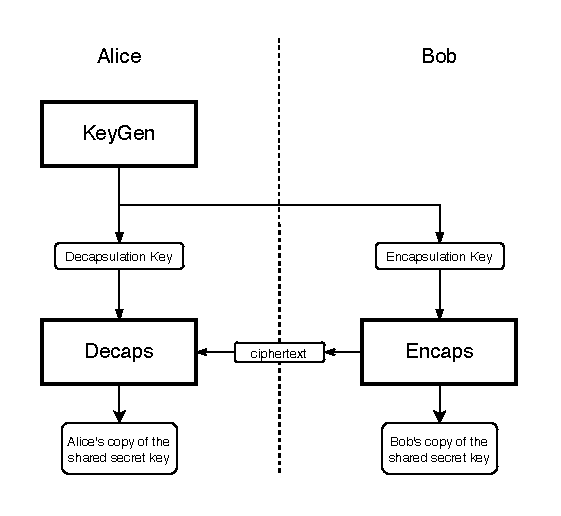
\includegraphics[width=0.5\textwidth]{doc/graph/KEM.drawio.pdf}
  \caption{KEM 工作流程图}
\end{figure}

由于 KEM 在 Decaps 阶段生成的共享密钥是确定性的,因此 KEM 通常会在 Encaps 阶段引入随机性,以避免密文的重放攻击。不同的 KEM 实现可能导致 Decaps 无法生成共享密钥,导致密文无法解密,通常会选择合适的参数,以保证发生这种情况的概率足够小。
% \section{MSKE 安全模型简述}

在密码学研究中,安全模型通常指导加密方案的设计,确保它们满足特定安全目标,并提供方案的执行框架。

Fischlin 等人在论文\cite{fischlin_multi-stage_2014}中提出多阶段密钥交换(Multi-Stage Key Exchange,MSKE)的安全模型,参考论文\cite{ideal_lattice_2023}及论文\cite{timke_2024}简要介绍如下:

MSKE 模型下参与者身份集表示为 $\mathcal{U}$,并且每一个 $U\in \mathcal{U}$ 有一个长期公钥 $\mathrm{pk}_{U}$ 和对应的私钥 $\mathrm{sk}_{U}$。 列表 $List_S$ 维护着所有会话信息,并由标签 $label$ 作为会话元组 $T$ 的唯一标识,$T$ = ($label$, $U$, $V$, $role$, $auth$, st$_\text{exec}$, $sID$, $K$, st$_{\text {key}}$, $tested$)。

其中 $U$ 与 $V$ 表示通信双方身份,
$role$ $\in\{ initiator, responder \}$ 记录会话所有者的角色。 
$auth$ 标识密钥交换协议的每个阶段的认证模式。
$\mathrm{st}_{\text{exec}}$[$label$, $i$]$\in$ \{running, accepted, rejected\} 表示在会话 $label$ 中第 $i$ 阶段的状态。 
sID 表示为针对阶段性的会话标识符,其中 $sID_i$ 表示第 $i$(非0)阶段中的会话标识符。
$K$ 表示会话 $label$ 在 $i$ 阶段中的阶段会话密钥。 
st$_\text{Key}$[$label$, $i$] $\in\{\text {fresh, revealed}\}$ 表示在会话 $label$ 中第 $i \neq 0 $ 阶段中会话(临时)密钥的状态。 
tested 记录会话密钥测试状态,$tested_i = true$ 则说明第 $i$ 阶段下的会话(临时)密钥已完成测试。

在 MSKE 安全模型下, 不允许临时密钥以及内部值(如服务器预共享密钥)泄露。 考虑一个 PPT 的敌手 $\mathcal{A}$,它控制着所有参与方之间的通信, 可以拦截、注入和丢弃消息。

\textbf{攻击手段. }敌手 $\mathcal{A}$ 通过以下查询与协议交互: 

\begin{itemize}
\setlength\itemsep{-0.3em}
\item NewSession($U$, $V$, $role$, $auth$): 为 $U$ 创建新的会话,角色为 $role$, 预期伙伴为$V$,身份验证类型 $auth$ $\in \{\text{unauth, unilateral, mutual}\}$
\item Send($label$, $m$): 发送消息$m$给标签为$label$的会话
\item Reveal($label$, $i$): 暴露$label$会话中第$i$阶段的会话密钥
\item Cor($U$): 攻陷用户$U$, 向敌手提供用户$U$长期公钥$\mathrm{pk}_{U}$ 对应的长期私钥,返回$\left(\mathrm{sk}_{U}, \mathrm{pk}_{U}\right)$
\item TEST($label$, $i$): 测试标签为 $label$ 的会话中第 $i$ 阶段的会话密钥
\end{itemize}
\subsection{TIMKE性能评估}

本节对不同配置下的TIMKE协议进行性能评估,分析各核心组件对整体性能的影响,并探讨保持安全性下的优化策略,为实际部署决策提供参考。

\subsubsection{评估方法}

实现提供一套性能评估框架,对协议各组件及其组合进行系统测试,包括:1)组件级基准测试,重点评估各KEM实现的关键操作(密钥生成、封装和解封装)性能,识别潜在瓶颈;2)协议阶段评估,分别测量第一阶段(包含0-RTT)和第二阶段的执行时间与资源消耗;3)端到端性能分析,评估完整协议流程的时间效率、内存占用和通信开销,模拟真实应用场景。替代实现对比则测试不同KEM组合的性能差异,分析最佳配置方案。

所有测试在统一的环境中进行,硬件平台为Apple M1 Pro (8核心CPU,16GB RAM),操作系统为MacOS Sequoia 15,开发语言为Go 1.23.4。每项测试重复10次取平均值,消除随机波动。测试工具集成于协议代码库,确保测量的准确性与一致性,不同身份的参与方会占用同一设备不同的端口进行交互。
重点测试两套KEM组合配置方案:1)理论构造配置使用OW-ChCCA KEM作为KEM\textsubscript{1}和ML-KEM作为KEM\textsubscript{2},代表原始TIMKE协议设计;2)实用替代配置使用ML-KEM同时作为KEM\textsubscript{1}和KEM\textsubscript{2},探索在当前技术条件下的最佳性能方案。

\subsubsection{混合KEM实现性能分析}

考虑到OW-ChCCA KEM的性能受限,首先评估折中方案:使用高度简化的OW-ChCCA变体(OWChCCA-mini)作为KEM\textsubscript{1},结合ML-KEM作为KEM\textsubscript{2}。OWChCCA-mini使用极小矩阵维度(n=16, m=8192, $\lambda$=16)和高度优化的算法实现。该配置仅作为概念验证使用,不应在实际安全系统中部署,仅提供理论构造可行性的基准数据。

\begin{table}[ht]
\centering
\caption{混合KEM实现的TIMKE协议性能(单位:毫秒)}
\label{tab:timke-hybrid-perf}
\begin{tabular}{|l|r|r|r|r|}
\hline
\textbf{KEM组合} & \textbf{阶段1} & \textbf{阶段2} & \textbf{总时间} & \textbf{内存(KB)} \\
\hline
OWChCCA-mini + ML-KEM-512    & 322.18  & 118.53  & 440.71  & 2,206,372   \\
\hline
OWChCCA-mini + ML-KEM-768    & 324.47  & 117.61  & 442.07  & 2,206,250   \\
\hline
OWChCCA-mini + ML-KEM-1024   & 374.76  & 127.47  & 502.23  & 2,204,554   \\
\hline
\end{tabular}
\end{table}

即使采用极度简化的OW-ChCCA变体,混合方案的性能仍然受到限制,不同配置总执行时间分别为440.71ms、442.07ms和502.23ms,在不稳定的网络环境下有更明显的延迟感知。第一阶段(使用OWChCCA-mini)执行时间占总时间的73\%至75\%,明确指出性能瓶颈所在。在高安全级别下更为明显,如OWChCCA-mini与ML-KEM-1024组合的配置中,第一阶段耗时达到374.76ms,几乎是第二阶段的3倍。所有混合配置均需要超过2GB的内存,远超移动设备和嵌入式系统的可用资源。较差的性能表现主要源于OWChCCA-mini中的矩阵运算,尽管较大程度的简化参数设置,但基本的LWE问题结构仍然导致过多的内存开销。

数据表明,尽管混合KEM方案在理论上实现了TIMKE协议的设计目标,但其实际性能表现使其难以直接应用于对延迟敏感的现代通信系统。

\subsubsection{ML-KEM替代实现性能分析}

本小节将分析使用ML-KEM同时替代KEM\textsubscript{1}和KEM\textsubscript{2}的方案。这种配置在理论上可能不提供与原设计相同的紧致安全保证,但为评估TIMKE协议在实际环境中的可行性提供了参考。

表\ref{tab:timke-mlkem-perf}展示了使用ML-KEM不同安全级别实现的TIMKE协议性能。

\begin{table}[ht]
\centering
\caption{基于ML-KEM的TIMKE协议性能(单位:毫秒)}
\label{tab:timke-mlkem-perf}
\begin{tabular}{|l|r|r|r|r|}
\hline
\textbf{KEM组合} & \textbf{阶段1} & \textbf{阶段2} & \textbf{总时间} & \textbf{内存(KB)} \\
\hline
ML-KEM-512 + ML-KEM-512    & 0.10  & 0.07  & 0.17  & 26   \\
\hline
ML-KEM-768 + ML-KEM-768    & 0.15  & 0.10  & 0.25  & 40   \\
\hline
ML-KEM-1024 + ML-KEM-1024  & 0.21  & 0.14  & 0.35  & 59   \\
\hline
\end{tabular}
\end{table}

在统一测试基准下,基于ML-KEM的配置比混合KEM方案快约3000倍。即使是安全级别最高的ML-KEM-1024配置,总执行时间也仅为0.35毫秒,完全满足高性能网络应用的需求。如此大的差距主要因为ML-KEM高效的算法结构和实现上的优化。ML-KEM基于模格结构,能够利用数论变换(NTT)等方式加速计算,其参数设置也经过精心优化,在保持安全的同时最小化计算开销。

内存使用方面,ML-KEM方案表现优秀。测试配置的内存消耗分别为26KB、40KB和59KB,比混合方案低4-5个数量级,使TIMKE协议能够在资源受限的环境中运行,如移动设备、物联网终端甚至某些嵌入式系统。低内存占用也意味着更低的能耗和更好的并发性能,对服务器端的部署尤为重要。

通信开销方面,基于ML-KEM的配置表现出色。ClientHello消息大小约为2-3KB,ServerResponse约为1-2KB,总通信量控制在5KB以内。阶段时间分布也更加均衡,第一阶段和第二阶段分别占总时间的约60\%和40\%。平均的时间分布在保证了0-RTT数据传输的低延迟特性的同时,不为后续阶段引入较大的额外延迟。

\paragraph{安全性降级影响分析}
从安全模型角度,OW-ChCCA安全专为紧致安全多挑战多用户场景设计,其安全损失与用户数量$n$和会话数量$q_s$无关,安全规约损失为常数$\mathcal{O}(1)$。ML-KEM虽然提供了IND-CCA2安全,但在多用户环境下其安全损失会随用户数量增加,典型的安全损失为$\mathcal{O}(n \cdot q_s)$。
对于小规模系统(如用户数$n < 10^3$,每用户会话数$q_s < 10^3$),ML-KEM配置下的安全性损失可接受,实际参数选择与理论安全级别差距可控;对于中等规模系统(如用户数$n \approx 10^6$,每用户会话数$q_s \approx 10^3$),安全损失达到$\mathcal{O}(10^9)$量级,需要增加密钥长度(约30比特)才能维持原有安全级别;对于大规模系统(如用户数$n > 10^8$,每用户会话数$q_s > 10^4$),安全损失将超过$\mathcal{O}(10^{12})$量级,安全参数增加需求可能使方案在计算和通信效率上不再具有实用性。

使用ML-KEM替代OW-ChCCA KEM作为KEM\textsubscript{1}会对TIMKE协议的整体安全性产生影响,具体如下:

\begin{enumerate}
    \item \textbf{紧致安全性}:完全失去紧致安全保证,安全损失会随系统规模增长。
    
    \item \textbf{后量子安全性}:保持不变,ML-KEM本身具有抗量子计算攻击能力。
    
    \item \textbf{0-RTT安全性}:基本保持,但在大规模部署中,可能需要增加密钥长度以补偿安全损失。
    
    \item \textbf{弱前向安全性}:第二阶段的弱前向安全性基本保持,因为它主要依赖于KEM\textsubscript{2}的安全性。
\end{enumerate}

综合来看,ML-KEM替代方案在部署TIMKE协议的中小规模系统中可以接受,安全降级影响有限。大规模部署环境则需权衡效率与安全性,可能要求更高安全级别的参数以补偿紧致安全性的损失。
\appendix
\ctexset { section = { name={附录},number={\Alph {section}}, format={\centering \zihao {-2}\bfseries } } } 
\titleformat{\subsection}{\zihao{-3}\bfseries}{\thesubsection}{1em}{}
\titleformat{\subsubsection}{\zihao{4}\bfseries}{\thesubsubsection}{1em}{}
\ctexset { paragraph = { ,format={\raggedright \bfseries \zihao {-4}} } }
\pagestyle{fancy}
\fancyhf{}
\renewcommand{\sectionmark}[1]{\markboth{附录\Alph{section}\ \ #1}{}}
\fancyhead[C]{\thesistitlefancyhead{}} % 页眉设置为论文标题
\fancyfoot[C]{\thepage}
\makeatletter
\@addtoreset{equation}{section}
\makeatother
\renewcommand{\theequation}{\Alph{section}.\arabic{equation}}
\section{密钥封装机制(KEM)概述}

KEM 是一种基于公钥密码学的密钥交换机制,使得通信双方可以在一定条件下构建共享秘密密钥,可以使用在接下来的对称加密环节。

一个 KEM 主要由三部分组成,分别是
\begin{itemize}
  \item KeyGen:概率性算法,生成公私钥对。
  \item Encaps:概率性算法,生成密文和共享密钥。
  \item Decaps:确定性算法,根据密文和私钥生成共享密钥。
\end{itemize}

\begin{figure}[ht]
  \centering
  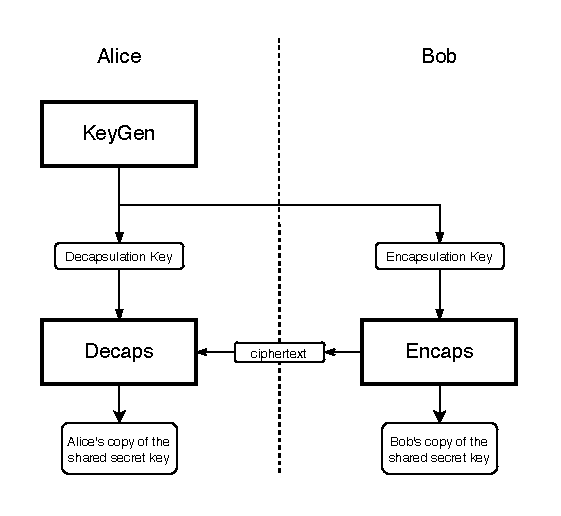
\includegraphics[width=0.5\textwidth]{doc/graph/KEM.drawio.pdf}
  \caption{KEM 工作流程图}
\end{figure}

由于 KEM 在 Decaps 阶段生成的共享密钥是确定性的,因此 KEM 通常会在 Encaps 阶段引入随机性,以避免密文的重放攻击。不同的 KEM 实现可能导致 Decaps 无法生成共享密钥,导致密文无法解密,通常会选择合适的参数,以保证发生这种情况的概率足够小。
% \section{MSKE 安全模型简述}

在密码学研究中,安全模型通常指导加密方案的设计,确保它们满足特定安全目标,并提供方案的执行框架。

Fischlin 等人在论文\cite{fischlin_multi-stage_2014}中提出多阶段密钥交换(Multi-Stage Key Exchange,MSKE)的安全模型,参考论文\cite{ideal_lattice_2023}及论文\cite{timke_2024}简要介绍如下:

MSKE 模型下参与者身份集表示为 $\mathcal{U}$,并且每一个 $U\in \mathcal{U}$ 有一个长期公钥 $\mathrm{pk}_{U}$ 和对应的私钥 $\mathrm{sk}_{U}$。 列表 $List_S$ 维护着所有会话信息,并由标签 $label$ 作为会话元组 $T$ 的唯一标识,$T$ = ($label$, $U$, $V$, $role$, $auth$, st$_\text{exec}$, $sID$, $K$, st$_{\text {key}}$, $tested$)。

其中 $U$ 与 $V$ 表示通信双方身份,
$role$ $\in\{ initiator, responder \}$ 记录会话所有者的角色。 
$auth$ 标识密钥交换协议的每个阶段的认证模式。
$\mathrm{st}_{\text{exec}}$[$label$, $i$]$\in$ \{running, accepted, rejected\} 表示在会话 $label$ 中第 $i$ 阶段的状态。 
sID 表示为针对阶段性的会话标识符,其中 $sID_i$ 表示第 $i$(非0)阶段中的会话标识符。
$K$ 表示会话 $label$ 在 $i$ 阶段中的阶段会话密钥。 
st$_\text{Key}$[$label$, $i$] $\in\{\text {fresh, revealed}\}$ 表示在会话 $label$ 中第 $i \neq 0 $ 阶段中会话(临时)密钥的状态。 
tested 记录会话密钥测试状态,$tested_i = true$ 则说明第 $i$ 阶段下的会话(临时)密钥已完成测试。

在 MSKE 安全模型下, 不允许临时密钥以及内部值(如服务器预共享密钥)泄露。 考虑一个 PPT 的敌手 $\mathcal{A}$,它控制着所有参与方之间的通信, 可以拦截、注入和丢弃消息。

\textbf{攻击手段. }敌手 $\mathcal{A}$ 通过以下查询与协议交互: 

\begin{itemize}
\setlength\itemsep{-0.3em}
\item NewSession($U$, $V$, $role$, $auth$): 为 $U$ 创建新的会话,角色为 $role$, 预期伙伴为$V$,身份验证类型 $auth$ $\in \{\text{unauth, unilateral, mutual}\}$
\item Send($label$, $m$): 发送消息$m$给标签为$label$的会话
\item Reveal($label$, $i$): 暴露$label$会话中第$i$阶段的会话密钥
\item Cor($U$): 攻陷用户$U$, 向敌手提供用户$U$长期公钥$\mathrm{pk}_{U}$ 对应的长期私钥,返回$\left(\mathrm{sk}_{U}, \mathrm{pk}_{U}\right)$
\item TEST($label$, $i$): 测试标签为 $label$ 的会话中第 $i$ 阶段的会话密钥
\end{itemize}
\subsection{TIMKE性能评估}

本节对不同配置下的TIMKE协议进行性能评估,分析各核心组件对整体性能的影响,并探讨保持安全性下的优化策略,为实际部署决策提供参考。

\subsubsection{评估方法}

实现提供一套性能评估框架,对协议各组件及其组合进行系统测试,包括:1)组件级基准测试,重点评估各KEM实现的关键操作(密钥生成、封装和解封装)性能,识别潜在瓶颈;2)协议阶段评估,分别测量第一阶段(包含0-RTT)和第二阶段的执行时间与资源消耗;3)端到端性能分析,评估完整协议流程的时间效率、内存占用和通信开销,模拟真实应用场景。替代实现对比则测试不同KEM组合的性能差异,分析最佳配置方案。

所有测试在统一的环境中进行,硬件平台为Apple M1 Pro (8核心CPU,16GB RAM),操作系统为MacOS Sequoia 15,开发语言为Go 1.23.4。每项测试重复10次取平均值,消除随机波动。测试工具集成于协议代码库,确保测量的准确性与一致性,不同身份的参与方会占用同一设备不同的端口进行交互。
重点测试两套KEM组合配置方案:1)理论构造配置使用OW-ChCCA KEM作为KEM\textsubscript{1}和ML-KEM作为KEM\textsubscript{2},代表原始TIMKE协议设计;2)实用替代配置使用ML-KEM同时作为KEM\textsubscript{1}和KEM\textsubscript{2},探索在当前技术条件下的最佳性能方案。

\subsubsection{混合KEM实现性能分析}

考虑到OW-ChCCA KEM的性能受限,首先评估折中方案:使用高度简化的OW-ChCCA变体(OWChCCA-mini)作为KEM\textsubscript{1},结合ML-KEM作为KEM\textsubscript{2}。OWChCCA-mini使用极小矩阵维度(n=16, m=8192, $\lambda$=16)和高度优化的算法实现。该配置仅作为概念验证使用,不应在实际安全系统中部署,仅提供理论构造可行性的基准数据。

\begin{table}[ht]
\centering
\caption{混合KEM实现的TIMKE协议性能(单位:毫秒)}
\label{tab:timke-hybrid-perf}
\begin{tabular}{|l|r|r|r|r|}
\hline
\textbf{KEM组合} & \textbf{阶段1} & \textbf{阶段2} & \textbf{总时间} & \textbf{内存(KB)} \\
\hline
OWChCCA-mini + ML-KEM-512    & 322.18  & 118.53  & 440.71  & 2,206,372   \\
\hline
OWChCCA-mini + ML-KEM-768    & 324.47  & 117.61  & 442.07  & 2,206,250   \\
\hline
OWChCCA-mini + ML-KEM-1024   & 374.76  & 127.47  & 502.23  & 2,204,554   \\
\hline
\end{tabular}
\end{table}

即使采用极度简化的OW-ChCCA变体,混合方案的性能仍然受到限制,不同配置总执行时间分别为440.71ms、442.07ms和502.23ms,在不稳定的网络环境下有更明显的延迟感知。第一阶段(使用OWChCCA-mini)执行时间占总时间的73\%至75\%,明确指出性能瓶颈所在。在高安全级别下更为明显,如OWChCCA-mini与ML-KEM-1024组合的配置中,第一阶段耗时达到374.76ms,几乎是第二阶段的3倍。所有混合配置均需要超过2GB的内存,远超移动设备和嵌入式系统的可用资源。较差的性能表现主要源于OWChCCA-mini中的矩阵运算,尽管较大程度的简化参数设置,但基本的LWE问题结构仍然导致过多的内存开销。

数据表明,尽管混合KEM方案在理论上实现了TIMKE协议的设计目标,但其实际性能表现使其难以直接应用于对延迟敏感的现代通信系统。

\subsubsection{ML-KEM替代实现性能分析}

本小节将分析使用ML-KEM同时替代KEM\textsubscript{1}和KEM\textsubscript{2}的方案。这种配置在理论上可能不提供与原设计相同的紧致安全保证,但为评估TIMKE协议在实际环境中的可行性提供了参考。

表\ref{tab:timke-mlkem-perf}展示了使用ML-KEM不同安全级别实现的TIMKE协议性能。

\begin{table}[ht]
\centering
\caption{基于ML-KEM的TIMKE协议性能(单位:毫秒)}
\label{tab:timke-mlkem-perf}
\begin{tabular}{|l|r|r|r|r|}
\hline
\textbf{KEM组合} & \textbf{阶段1} & \textbf{阶段2} & \textbf{总时间} & \textbf{内存(KB)} \\
\hline
ML-KEM-512 + ML-KEM-512    & 0.10  & 0.07  & 0.17  & 26   \\
\hline
ML-KEM-768 + ML-KEM-768    & 0.15  & 0.10  & 0.25  & 40   \\
\hline
ML-KEM-1024 + ML-KEM-1024  & 0.21  & 0.14  & 0.35  & 59   \\
\hline
\end{tabular}
\end{table}

在统一测试基准下,基于ML-KEM的配置比混合KEM方案快约3000倍。即使是安全级别最高的ML-KEM-1024配置,总执行时间也仅为0.35毫秒,完全满足高性能网络应用的需求。如此大的差距主要因为ML-KEM高效的算法结构和实现上的优化。ML-KEM基于模格结构,能够利用数论变换(NTT)等方式加速计算,其参数设置也经过精心优化,在保持安全的同时最小化计算开销。

内存使用方面,ML-KEM方案表现优秀。测试配置的内存消耗分别为26KB、40KB和59KB,比混合方案低4-5个数量级,使TIMKE协议能够在资源受限的环境中运行,如移动设备、物联网终端甚至某些嵌入式系统。低内存占用也意味着更低的能耗和更好的并发性能,对服务器端的部署尤为重要。

通信开销方面,基于ML-KEM的配置表现出色。ClientHello消息大小约为2-3KB,ServerResponse约为1-2KB,总通信量控制在5KB以内。阶段时间分布也更加均衡,第一阶段和第二阶段分别占总时间的约60\%和40\%。平均的时间分布在保证了0-RTT数据传输的低延迟特性的同时,不为后续阶段引入较大的额外延迟。

\paragraph{安全性降级影响分析}
从安全模型角度,OW-ChCCA安全专为紧致安全多挑战多用户场景设计,其安全损失与用户数量$n$和会话数量$q_s$无关,安全规约损失为常数$\mathcal{O}(1)$。ML-KEM虽然提供了IND-CCA2安全,但在多用户环境下其安全损失会随用户数量增加,典型的安全损失为$\mathcal{O}(n \cdot q_s)$。
对于小规模系统(如用户数$n < 10^3$,每用户会话数$q_s < 10^3$),ML-KEM配置下的安全性损失可接受,实际参数选择与理论安全级别差距可控;对于中等规模系统(如用户数$n \approx 10^6$,每用户会话数$q_s \approx 10^3$),安全损失达到$\mathcal{O}(10^9)$量级,需要增加密钥长度(约30比特)才能维持原有安全级别;对于大规模系统(如用户数$n > 10^8$,每用户会话数$q_s > 10^4$),安全损失将超过$\mathcal{O}(10^{12})$量级,安全参数增加需求可能使方案在计算和通信效率上不再具有实用性。

使用ML-KEM替代OW-ChCCA KEM作为KEM\textsubscript{1}会对TIMKE协议的整体安全性产生影响,具体如下:

\begin{enumerate}
    \item \textbf{紧致安全性}:完全失去紧致安全保证,安全损失会随系统规模增长。
    
    \item \textbf{后量子安全性}:保持不变,ML-KEM本身具有抗量子计算攻击能力。
    
    \item \textbf{0-RTT安全性}:基本保持,但在大规模部署中,可能需要增加密钥长度以补偿安全损失。
    
    \item \textbf{弱前向安全性}:第二阶段的弱前向安全性基本保持,因为它主要依赖于KEM\textsubscript{2}的安全性。
\end{enumerate}

综合来看,ML-KEM替代方案在部署TIMKE协议的中小规模系统中可以接受,安全降级影响有限。大规模部署环境则需权衡效率与安全性,可能要求更高安全级别的参数以补偿紧致安全性的损失。
\appendix
\ctexset { section = { name={附录},number={\Alph {section}}, format={\centering \zihao {-2}\bfseries } } } 
\titleformat{\subsection}{\zihao{-3}\bfseries}{\thesubsection}{1em}{}
\titleformat{\subsubsection}{\zihao{4}\bfseries}{\thesubsubsection}{1em}{}
\ctexset { paragraph = { ,format={\raggedright \bfseries \zihao {-4}} } }
\pagestyle{fancy}
\fancyhf{}
\renewcommand{\sectionmark}[1]{\markboth{附录\Alph{section}\ \ #1}{}}
\fancyhead[C]{\thesistitlefancyhead{}} % 页眉设置为论文标题
\fancyfoot[C]{\thepage}
\makeatletter
\@addtoreset{equation}{section}
\makeatother
\renewcommand{\theequation}{\Alph{section}.\arabic{equation}}
\section{密钥封装机制(KEM)概述}

KEM 是一种基于公钥密码学的密钥交换机制,使得通信双方可以在一定条件下构建共享秘密密钥,可以使用在接下来的对称加密环节。

一个 KEM 主要由三部分组成,分别是
\begin{itemize}
  \item KeyGen:概率性算法,生成公私钥对。
  \item Encaps:概率性算法,生成密文和共享密钥。
  \item Decaps:确定性算法,根据密文和私钥生成共享密钥。
\end{itemize}

\begin{figure}[ht]
  \centering
  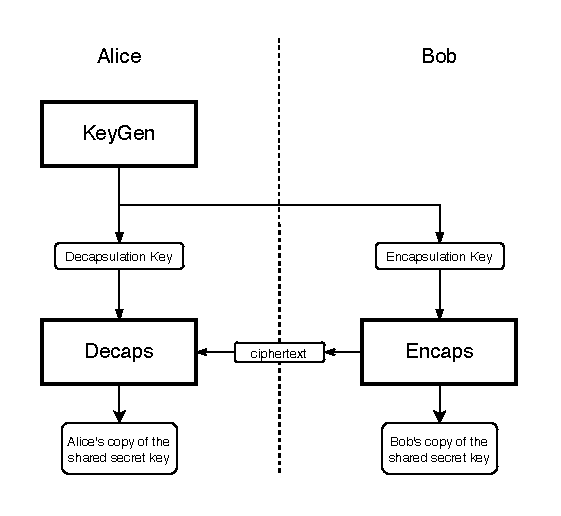
\includegraphics[width=0.5\textwidth]{doc/graph/KEM.drawio.pdf}
  \caption{KEM 工作流程图}
\end{figure}

由于 KEM 在 Decaps 阶段生成的共享密钥是确定性的,因此 KEM 通常会在 Encaps 阶段引入随机性,以避免密文的重放攻击。不同的 KEM 实现可能导致 Decaps 无法生成共享密钥,导致密文无法解密,通常会选择合适的参数,以保证发生这种情况的概率足够小。
% \section{MSKE 安全模型简述}

在密码学研究中,安全模型通常指导加密方案的设计,确保它们满足特定安全目标,并提供方案的执行框架。

Fischlin 等人在论文\cite{fischlin_multi-stage_2014}中提出多阶段密钥交换(Multi-Stage Key Exchange,MSKE)的安全模型,参考论文\cite{ideal_lattice_2023}及论文\cite{timke_2024}简要介绍如下:

MSKE 模型下参与者身份集表示为 $\mathcal{U}$,并且每一个 $U\in \mathcal{U}$ 有一个长期公钥 $\mathrm{pk}_{U}$ 和对应的私钥 $\mathrm{sk}_{U}$。 列表 $List_S$ 维护着所有会话信息,并由标签 $label$ 作为会话元组 $T$ 的唯一标识,$T$ = ($label$, $U$, $V$, $role$, $auth$, st$_\text{exec}$, $sID$, $K$, st$_{\text {key}}$, $tested$)。

其中 $U$ 与 $V$ 表示通信双方身份,
$role$ $\in\{ initiator, responder \}$ 记录会话所有者的角色。 
$auth$ 标识密钥交换协议的每个阶段的认证模式。
$\mathrm{st}_{\text{exec}}$[$label$, $i$]$\in$ \{running, accepted, rejected\} 表示在会话 $label$ 中第 $i$ 阶段的状态。 
sID 表示为针对阶段性的会话标识符,其中 $sID_i$ 表示第 $i$(非0)阶段中的会话标识符。
$K$ 表示会话 $label$ 在 $i$ 阶段中的阶段会话密钥。 
st$_\text{Key}$[$label$, $i$] $\in\{\text {fresh, revealed}\}$ 表示在会话 $label$ 中第 $i \neq 0 $ 阶段中会话(临时)密钥的状态。 
tested 记录会话密钥测试状态,$tested_i = true$ 则说明第 $i$ 阶段下的会话(临时)密钥已完成测试。

在 MSKE 安全模型下, 不允许临时密钥以及内部值(如服务器预共享密钥)泄露。 考虑一个 PPT 的敌手 $\mathcal{A}$,它控制着所有参与方之间的通信, 可以拦截、注入和丢弃消息。

\textbf{攻击手段. }敌手 $\mathcal{A}$ 通过以下查询与协议交互: 

\begin{itemize}
\setlength\itemsep{-0.3em}
\item NewSession($U$, $V$, $role$, $auth$): 为 $U$ 创建新的会话,角色为 $role$, 预期伙伴为$V$,身份验证类型 $auth$ $\in \{\text{unauth, unilateral, mutual}\}$
\item Send($label$, $m$): 发送消息$m$给标签为$label$的会话
\item Reveal($label$, $i$): 暴露$label$会话中第$i$阶段的会话密钥
\item Cor($U$): 攻陷用户$U$, 向敌手提供用户$U$长期公钥$\mathrm{pk}_{U}$ 对应的长期私钥,返回$\left(\mathrm{sk}_{U}, \mathrm{pk}_{U}\right)$
\item TEST($label$, $i$): 测试标签为 $label$ 的会话中第 $i$ 阶段的会话密钥
\end{itemize}
\subsection{TIMKE性能评估}

本节对不同配置下的TIMKE协议进行性能评估,分析各核心组件对整体性能的影响,并探讨保持安全性下的优化策略,为实际部署决策提供参考。

\subsubsection{评估方法}

实现提供一套性能评估框架,对协议各组件及其组合进行系统测试,包括:1)组件级基准测试,重点评估各KEM实现的关键操作(密钥生成、封装和解封装)性能,识别潜在瓶颈;2)协议阶段评估,分别测量第一阶段(包含0-RTT)和第二阶段的执行时间与资源消耗;3)端到端性能分析,评估完整协议流程的时间效率、内存占用和通信开销,模拟真实应用场景。替代实现对比则测试不同KEM组合的性能差异,分析最佳配置方案。

所有测试在统一的环境中进行,硬件平台为Apple M1 Pro (8核心CPU,16GB RAM),操作系统为MacOS Sequoia 15,开发语言为Go 1.23.4。每项测试重复10次取平均值,消除随机波动。测试工具集成于协议代码库,确保测量的准确性与一致性,不同身份的参与方会占用同一设备不同的端口进行交互。
重点测试两套KEM组合配置方案:1)理论构造配置使用OW-ChCCA KEM作为KEM\textsubscript{1}和ML-KEM作为KEM\textsubscript{2},代表原始TIMKE协议设计;2)实用替代配置使用ML-KEM同时作为KEM\textsubscript{1}和KEM\textsubscript{2},探索在当前技术条件下的最佳性能方案。

\subsubsection{混合KEM实现性能分析}

考虑到OW-ChCCA KEM的性能受限,首先评估折中方案:使用高度简化的OW-ChCCA变体(OWChCCA-mini)作为KEM\textsubscript{1},结合ML-KEM作为KEM\textsubscript{2}。OWChCCA-mini使用极小矩阵维度(n=16, m=8192, $\lambda$=16)和高度优化的算法实现。该配置仅作为概念验证使用,不应在实际安全系统中部署,仅提供理论构造可行性的基准数据。

\begin{table}[ht]
\centering
\caption{混合KEM实现的TIMKE协议性能(单位:毫秒)}
\label{tab:timke-hybrid-perf}
\begin{tabular}{|l|r|r|r|r|}
\hline
\textbf{KEM组合} & \textbf{阶段1} & \textbf{阶段2} & \textbf{总时间} & \textbf{内存(KB)} \\
\hline
OWChCCA-mini + ML-KEM-512    & 322.18  & 118.53  & 440.71  & 2,206,372   \\
\hline
OWChCCA-mini + ML-KEM-768    & 324.47  & 117.61  & 442.07  & 2,206,250   \\
\hline
OWChCCA-mini + ML-KEM-1024   & 374.76  & 127.47  & 502.23  & 2,204,554   \\
\hline
\end{tabular}
\end{table}

即使采用极度简化的OW-ChCCA变体,混合方案的性能仍然受到限制,不同配置总执行时间分别为440.71ms、442.07ms和502.23ms,在不稳定的网络环境下有更明显的延迟感知。第一阶段(使用OWChCCA-mini)执行时间占总时间的73\%至75\%,明确指出性能瓶颈所在。在高安全级别下更为明显,如OWChCCA-mini与ML-KEM-1024组合的配置中,第一阶段耗时达到374.76ms,几乎是第二阶段的3倍。所有混合配置均需要超过2GB的内存,远超移动设备和嵌入式系统的可用资源。较差的性能表现主要源于OWChCCA-mini中的矩阵运算,尽管较大程度的简化参数设置,但基本的LWE问题结构仍然导致过多的内存开销。

数据表明,尽管混合KEM方案在理论上实现了TIMKE协议的设计目标,但其实际性能表现使其难以直接应用于对延迟敏感的现代通信系统。

\subsubsection{ML-KEM替代实现性能分析}

本小节将分析使用ML-KEM同时替代KEM\textsubscript{1}和KEM\textsubscript{2}的方案。这种配置在理论上可能不提供与原设计相同的紧致安全保证,但为评估TIMKE协议在实际环境中的可行性提供了参考。

表\ref{tab:timke-mlkem-perf}展示了使用ML-KEM不同安全级别实现的TIMKE协议性能。

\begin{table}[ht]
\centering
\caption{基于ML-KEM的TIMKE协议性能(单位:毫秒)}
\label{tab:timke-mlkem-perf}
\begin{tabular}{|l|r|r|r|r|}
\hline
\textbf{KEM组合} & \textbf{阶段1} & \textbf{阶段2} & \textbf{总时间} & \textbf{内存(KB)} \\
\hline
ML-KEM-512 + ML-KEM-512    & 0.10  & 0.07  & 0.17  & 26   \\
\hline
ML-KEM-768 + ML-KEM-768    & 0.15  & 0.10  & 0.25  & 40   \\
\hline
ML-KEM-1024 + ML-KEM-1024  & 0.21  & 0.14  & 0.35  & 59   \\
\hline
\end{tabular}
\end{table}

在统一测试基准下,基于ML-KEM的配置比混合KEM方案快约3000倍。即使是安全级别最高的ML-KEM-1024配置,总执行时间也仅为0.35毫秒,完全满足高性能网络应用的需求。如此大的差距主要因为ML-KEM高效的算法结构和实现上的优化。ML-KEM基于模格结构,能够利用数论变换(NTT)等方式加速计算,其参数设置也经过精心优化,在保持安全的同时最小化计算开销。

内存使用方面,ML-KEM方案表现优秀。测试配置的内存消耗分别为26KB、40KB和59KB,比混合方案低4-5个数量级,使TIMKE协议能够在资源受限的环境中运行,如移动设备、物联网终端甚至某些嵌入式系统。低内存占用也意味着更低的能耗和更好的并发性能,对服务器端的部署尤为重要。

通信开销方面,基于ML-KEM的配置表现出色。ClientHello消息大小约为2-3KB,ServerResponse约为1-2KB,总通信量控制在5KB以内。阶段时间分布也更加均衡,第一阶段和第二阶段分别占总时间的约60\%和40\%。平均的时间分布在保证了0-RTT数据传输的低延迟特性的同时,不为后续阶段引入较大的额外延迟。

\paragraph{安全性降级影响分析}
从安全模型角度,OW-ChCCA安全专为紧致安全多挑战多用户场景设计,其安全损失与用户数量$n$和会话数量$q_s$无关,安全规约损失为常数$\mathcal{O}(1)$。ML-KEM虽然提供了IND-CCA2安全,但在多用户环境下其安全损失会随用户数量增加,典型的安全损失为$\mathcal{O}(n \cdot q_s)$。
对于小规模系统(如用户数$n < 10^3$,每用户会话数$q_s < 10^3$),ML-KEM配置下的安全性损失可接受,实际参数选择与理论安全级别差距可控;对于中等规模系统(如用户数$n \approx 10^6$,每用户会话数$q_s \approx 10^3$),安全损失达到$\mathcal{O}(10^9)$量级,需要增加密钥长度(约30比特)才能维持原有安全级别;对于大规模系统(如用户数$n > 10^8$,每用户会话数$q_s > 10^4$),安全损失将超过$\mathcal{O}(10^{12})$量级,安全参数增加需求可能使方案在计算和通信效率上不再具有实用性。

使用ML-KEM替代OW-ChCCA KEM作为KEM\textsubscript{1}会对TIMKE协议的整体安全性产生影响,具体如下:

\begin{enumerate}
    \item \textbf{紧致安全性}:完全失去紧致安全保证,安全损失会随系统规模增长。
    
    \item \textbf{后量子安全性}:保持不变,ML-KEM本身具有抗量子计算攻击能力。
    
    \item \textbf{0-RTT安全性}:基本保持,但在大规模部署中,可能需要增加密钥长度以补偿安全损失。
    
    \item \textbf{弱前向安全性}:第二阶段的弱前向安全性基本保持,因为它主要依赖于KEM\textsubscript{2}的安全性。
\end{enumerate}

综合来看,ML-KEM替代方案在部署TIMKE协议的中小规模系统中可以接受,安全降级影响有限。大规模部署环境则需权衡效率与安全性,可能要求更高安全级别的参数以补偿紧致安全性的损失。
\appendix
\ctexset { section = { name={附录},number={\Alph {section}}, format={\centering \zihao {-2}\bfseries } } } 
\titleformat{\subsection}{\zihao{-3}\bfseries}{\thesubsection}{1em}{}
\titleformat{\subsubsection}{\zihao{4}\bfseries}{\thesubsubsection}{1em}{}
\ctexset { paragraph = { ,format={\raggedright \bfseries \zihao {-4}} } }
\pagestyle{fancy}
\fancyhf{}
\renewcommand{\sectionmark}[1]{\markboth{附录\Alph{section}\ \ #1}{}}
\fancyhead[C]{\thesistitlefancyhead{}} % 页眉设置为论文标题
\fancyfoot[C]{\thepage}
\makeatletter
\@addtoreset{equation}{section}
\makeatother
\renewcommand{\theequation}{\Alph{section}.\arabic{equation}}
\section{密钥封装机制(KEM)概述}

KEM 是一种基于公钥密码学的密钥交换机制,使得通信双方可以在一定条件下构建共享秘密密钥,可以使用在接下来的对称加密环节。

一个 KEM 主要由三部分组成,分别是
\begin{itemize}
  \item KeyGen:概率性算法,生成公私钥对。
  \item Encaps:概率性算法,生成密文和共享密钥。
  \item Decaps:确定性算法,根据密文和私钥生成共享密钥。
\end{itemize}

\begin{figure}[ht]
  \centering
  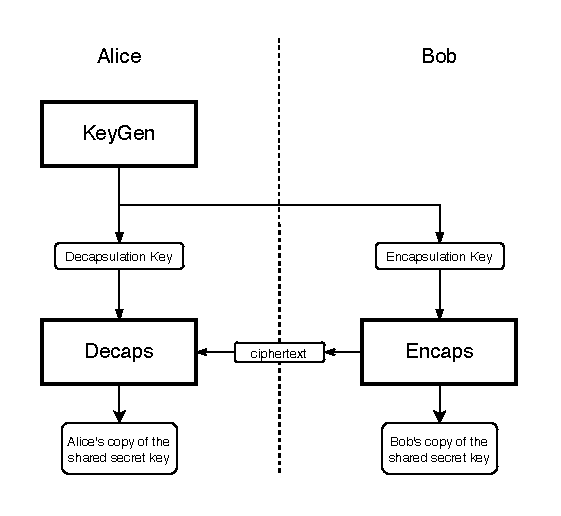
\includegraphics[width=0.5\textwidth]{doc/graph/KEM.drawio.pdf}
  \caption{KEM 工作流程图}
\end{figure}

由于 KEM 在 Decaps 阶段生成的共享密钥是确定性的,因此 KEM 通常会在 Encaps 阶段引入随机性,以避免密文的重放攻击。不同的 KEM 实现可能导致 Decaps 无法生成共享密钥,导致密文无法解密,通常会选择合适的参数,以保证发生这种情况的概率足够小。
% \section{MSKE 安全模型简述}

在密码学研究中,安全模型通常指导加密方案的设计,确保它们满足特定安全目标,并提供方案的执行框架。

Fischlin 等人在论文\cite{fischlin_multi-stage_2014}中提出多阶段密钥交换(Multi-Stage Key Exchange,MSKE)的安全模型,参考论文\cite{ideal_lattice_2023}及论文\cite{timke_2024}简要介绍如下:

MSKE 模型下参与者身份集表示为 $\mathcal{U}$,并且每一个 $U\in \mathcal{U}$ 有一个长期公钥 $\mathrm{pk}_{U}$ 和对应的私钥 $\mathrm{sk}_{U}$。 列表 $List_S$ 维护着所有会话信息,并由标签 $label$ 作为会话元组 $T$ 的唯一标识,$T$ = ($label$, $U$, $V$, $role$, $auth$, st$_\text{exec}$, $sID$, $K$, st$_{\text {key}}$, $tested$)。

其中 $U$ 与 $V$ 表示通信双方身份,
$role$ $\in\{ initiator, responder \}$ 记录会话所有者的角色。 
$auth$ 标识密钥交换协议的每个阶段的认证模式。
$\mathrm{st}_{\text{exec}}$[$label$, $i$]$\in$ \{running, accepted, rejected\} 表示在会话 $label$ 中第 $i$ 阶段的状态。 
sID 表示为针对阶段性的会话标识符,其中 $sID_i$ 表示第 $i$(非0)阶段中的会话标识符。
$K$ 表示会话 $label$ 在 $i$ 阶段中的阶段会话密钥。 
st$_\text{Key}$[$label$, $i$] $\in\{\text {fresh, revealed}\}$ 表示在会话 $label$ 中第 $i \neq 0 $ 阶段中会话(临时)密钥的状态。 
tested 记录会话密钥测试状态,$tested_i = true$ 则说明第 $i$ 阶段下的会话(临时)密钥已完成测试。

在 MSKE 安全模型下, 不允许临时密钥以及内部值(如服务器预共享密钥)泄露。 考虑一个 PPT 的敌手 $\mathcal{A}$,它控制着所有参与方之间的通信, 可以拦截、注入和丢弃消息。

\textbf{攻击手段. }敌手 $\mathcal{A}$ 通过以下查询与协议交互: 

\begin{itemize}
\setlength\itemsep{-0.3em}
\item NewSession($U$, $V$, $role$, $auth$): 为 $U$ 创建新的会话,角色为 $role$, 预期伙伴为$V$,身份验证类型 $auth$ $\in \{\text{unauth, unilateral, mutual}\}$
\item Send($label$, $m$): 发送消息$m$给标签为$label$的会话
\item Reveal($label$, $i$): 暴露$label$会话中第$i$阶段的会话密钥
\item Cor($U$): 攻陷用户$U$, 向敌手提供用户$U$长期公钥$\mathrm{pk}_{U}$ 对应的长期私钥,返回$\left(\mathrm{sk}_{U}, \mathrm{pk}_{U}\right)$
\item TEST($label$, $i$): 测试标签为 $label$ 的会话中第 $i$ 阶段的会话密钥
\end{itemize}
\subsection{TIMKE性能评估}

本节对不同配置下的TIMKE协议进行性能评估,分析各核心组件对整体性能的影响,并探讨保持安全性下的优化策略,为实际部署决策提供参考。

\subsubsection{评估方法}

实现提供一套性能评估框架,对协议各组件及其组合进行系统测试,包括:1)组件级基准测试,重点评估各KEM实现的关键操作(密钥生成、封装和解封装)性能,识别潜在瓶颈;2)协议阶段评估,分别测量第一阶段(包含0-RTT)和第二阶段的执行时间与资源消耗;3)端到端性能分析,评估完整协议流程的时间效率、内存占用和通信开销,模拟真实应用场景。替代实现对比则测试不同KEM组合的性能差异,分析最佳配置方案。

所有测试在统一的环境中进行,硬件平台为Apple M1 Pro (8核心CPU,16GB RAM),操作系统为MacOS Sequoia 15,开发语言为Go 1.23.4。每项测试重复10次取平均值,消除随机波动。测试工具集成于协议代码库,确保测量的准确性与一致性,不同身份的参与方会占用同一设备不同的端口进行交互。
重点测试两套KEM组合配置方案:1)理论构造配置使用OW-ChCCA KEM作为KEM\textsubscript{1}和ML-KEM作为KEM\textsubscript{2},代表原始TIMKE协议设计;2)实用替代配置使用ML-KEM同时作为KEM\textsubscript{1}和KEM\textsubscript{2},探索在当前技术条件下的最佳性能方案。

\subsubsection{混合KEM实现性能分析}

考虑到OW-ChCCA KEM的性能受限,首先评估折中方案:使用高度简化的OW-ChCCA变体(OWChCCA-mini)作为KEM\textsubscript{1},结合ML-KEM作为KEM\textsubscript{2}。OWChCCA-mini使用极小矩阵维度(n=16, m=8192, $\lambda$=16)和高度优化的算法实现。该配置仅作为概念验证使用,不应在实际安全系统中部署,仅提供理论构造可行性的基准数据。

\begin{table}[ht]
\centering
\caption{混合KEM实现的TIMKE协议性能(单位:毫秒)}
\label{tab:timke-hybrid-perf}
\begin{tabular}{|l|r|r|r|r|}
\hline
\textbf{KEM组合} & \textbf{阶段1} & \textbf{阶段2} & \textbf{总时间} & \textbf{内存(KB)} \\
\hline
OWChCCA-mini + ML-KEM-512    & 322.18  & 118.53  & 440.71  & 2,206,372   \\
\hline
OWChCCA-mini + ML-KEM-768    & 324.47  & 117.61  & 442.07  & 2,206,250   \\
\hline
OWChCCA-mini + ML-KEM-1024   & 374.76  & 127.47  & 502.23  & 2,204,554   \\
\hline
\end{tabular}
\end{table}

即使采用极度简化的OW-ChCCA变体,混合方案的性能仍然受到限制,不同配置总执行时间分别为440.71ms、442.07ms和502.23ms,在不稳定的网络环境下有更明显的延迟感知。第一阶段(使用OWChCCA-mini)执行时间占总时间的73\%至75\%,明确指出性能瓶颈所在。在高安全级别下更为明显,如OWChCCA-mini与ML-KEM-1024组合的配置中,第一阶段耗时达到374.76ms,几乎是第二阶段的3倍。所有混合配置均需要超过2GB的内存,远超移动设备和嵌入式系统的可用资源。较差的性能表现主要源于OWChCCA-mini中的矩阵运算,尽管较大程度的简化参数设置,但基本的LWE问题结构仍然导致过多的内存开销。

数据表明,尽管混合KEM方案在理论上实现了TIMKE协议的设计目标,但其实际性能表现使其难以直接应用于对延迟敏感的现代通信系统。

\subsubsection{ML-KEM替代实现性能分析}

本小节将分析使用ML-KEM同时替代KEM\textsubscript{1}和KEM\textsubscript{2}的方案。这种配置在理论上可能不提供与原设计相同的紧致安全保证,但为评估TIMKE协议在实际环境中的可行性提供了参考。

表\ref{tab:timke-mlkem-perf}展示了使用ML-KEM不同安全级别实现的TIMKE协议性能。

\begin{table}[ht]
\centering
\caption{基于ML-KEM的TIMKE协议性能(单位:毫秒)}
\label{tab:timke-mlkem-perf}
\begin{tabular}{|l|r|r|r|r|}
\hline
\textbf{KEM组合} & \textbf{阶段1} & \textbf{阶段2} & \textbf{总时间} & \textbf{内存(KB)} \\
\hline
ML-KEM-512 + ML-KEM-512    & 0.10  & 0.07  & 0.17  & 26   \\
\hline
ML-KEM-768 + ML-KEM-768    & 0.15  & 0.10  & 0.25  & 40   \\
\hline
ML-KEM-1024 + ML-KEM-1024  & 0.21  & 0.14  & 0.35  & 59   \\
\hline
\end{tabular}
\end{table}

在统一测试基准下,基于ML-KEM的配置比混合KEM方案快约3000倍。即使是安全级别最高的ML-KEM-1024配置,总执行时间也仅为0.35毫秒,完全满足高性能网络应用的需求。如此大的差距主要因为ML-KEM高效的算法结构和实现上的优化。ML-KEM基于模格结构,能够利用数论变换(NTT)等方式加速计算,其参数设置也经过精心优化,在保持安全的同时最小化计算开销。

内存使用方面,ML-KEM方案表现优秀。测试配置的内存消耗分别为26KB、40KB和59KB,比混合方案低4-5个数量级,使TIMKE协议能够在资源受限的环境中运行,如移动设备、物联网终端甚至某些嵌入式系统。低内存占用也意味着更低的能耗和更好的并发性能,对服务器端的部署尤为重要。

通信开销方面,基于ML-KEM的配置表现出色。ClientHello消息大小约为2-3KB,ServerResponse约为1-2KB,总通信量控制在5KB以内。阶段时间分布也更加均衡,第一阶段和第二阶段分别占总时间的约60\%和40\%。平均的时间分布在保证了0-RTT数据传输的低延迟特性的同时,不为后续阶段引入较大的额外延迟。

\paragraph{安全性降级影响分析}
从安全模型角度,OW-ChCCA安全专为紧致安全多挑战多用户场景设计,其安全损失与用户数量$n$和会话数量$q_s$无关,安全规约损失为常数$\mathcal{O}(1)$。ML-KEM虽然提供了IND-CCA2安全,但在多用户环境下其安全损失会随用户数量增加,典型的安全损失为$\mathcal{O}(n \cdot q_s)$。
对于小规模系统(如用户数$n < 10^3$,每用户会话数$q_s < 10^3$),ML-KEM配置下的安全性损失可接受,实际参数选择与理论安全级别差距可控;对于中等规模系统(如用户数$n \approx 10^6$,每用户会话数$q_s \approx 10^3$),安全损失达到$\mathcal{O}(10^9)$量级,需要增加密钥长度(约30比特)才能维持原有安全级别;对于大规模系统(如用户数$n > 10^8$,每用户会话数$q_s > 10^4$),安全损失将超过$\mathcal{O}(10^{12})$量级,安全参数增加需求可能使方案在计算和通信效率上不再具有实用性。

使用ML-KEM替代OW-ChCCA KEM作为KEM\textsubscript{1}会对TIMKE协议的整体安全性产生影响,具体如下:

\begin{enumerate}
    \item \textbf{紧致安全性}:完全失去紧致安全保证,安全损失会随系统规模增长。
    
    \item \textbf{后量子安全性}:保持不变,ML-KEM本身具有抗量子计算攻击能力。
    
    \item \textbf{0-RTT安全性}:基本保持,但在大规模部署中,可能需要增加密钥长度以补偿安全损失。
    
    \item \textbf{弱前向安全性}:第二阶段的弱前向安全性基本保持,因为它主要依赖于KEM\textsubscript{2}的安全性。
\end{enumerate}

综合来看,ML-KEM替代方案在部署TIMKE协议的中小规模系统中可以接受,安全降级影响有限。大规模部署环境则需权衡效率与安全性,可能要求更高安全级别的参数以补偿紧致安全性的损失。
\appendix
\ctexset { section = { name={附录},number={\Alph {section}}, format={\centering \zihao {-2}\bfseries } } } 
\titleformat{\subsection}{\zihao{-3}\bfseries}{\thesubsection}{1em}{}
\titleformat{\subsubsection}{\zihao{4}\bfseries}{\thesubsubsection}{1em}{}
\ctexset { paragraph = { ,format={\raggedright \bfseries \zihao {-4}} } }
\pagestyle{fancy}
\fancyhf{}
\renewcommand{\sectionmark}[1]{\markboth{附录\Alph{section}\ \ #1}{}}
\fancyhead[C]{\thesistitlefancyhead{}} % 页眉设置为论文标题
\fancyfoot[C]{\thepage}
\makeatletter
\@addtoreset{equation}{section}
\makeatother
\renewcommand{\theequation}{\Alph{section}.\arabic{equation}}
\section{密钥封装机制(KEM)概述}

KEM 是一种基于公钥密码学的密钥交换机制,使得通信双方可以在一定条件下构建共享秘密密钥,可以使用在接下来的对称加密环节。

一个 KEM 主要由三部分组成,分别是
\begin{itemize}
  \item KeyGen:概率性算法,生成公私钥对。
  \item Encaps:概率性算法,生成密文和共享密钥。
  \item Decaps:确定性算法,根据密文和私钥生成共享密钥。
\end{itemize}

\begin{figure}[ht]
  \centering
  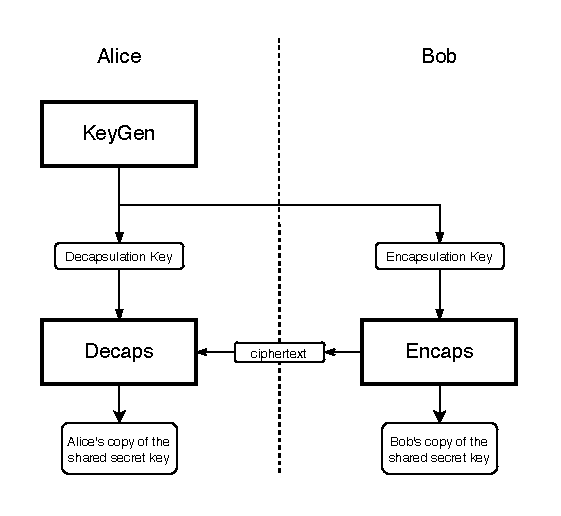
\includegraphics[width=0.5\textwidth]{doc/graph/KEM.drawio.pdf}
  \caption{KEM 工作流程图}
\end{figure}

由于 KEM 在 Decaps 阶段生成的共享密钥是确定性的,因此 KEM 通常会在 Encaps 阶段引入随机性,以避免密文的重放攻击。不同的 KEM 实现可能导致 Decaps 无法生成共享密钥,导致密文无法解密,通常会选择合适的参数,以保证发生这种情况的概率足够小。
% \section{MSKE 安全模型简述}

在密码学研究中,安全模型通常指导加密方案的设计,确保它们满足特定安全目标,并提供方案的执行框架。

Fischlin 等人在论文\cite{fischlin_multi-stage_2014}中提出多阶段密钥交换(Multi-Stage Key Exchange,MSKE)的安全模型,参考论文\cite{ideal_lattice_2023}及论文\cite{timke_2024}简要介绍如下:

MSKE 模型下参与者身份集表示为 $\mathcal{U}$,并且每一个 $U\in \mathcal{U}$ 有一个长期公钥 $\mathrm{pk}_{U}$ 和对应的私钥 $\mathrm{sk}_{U}$。 列表 $List_S$ 维护着所有会话信息,并由标签 $label$ 作为会话元组 $T$ 的唯一标识,$T$ = ($label$, $U$, $V$, $role$, $auth$, st$_\text{exec}$, $sID$, $K$, st$_{\text {key}}$, $tested$)。

其中 $U$ 与 $V$ 表示通信双方身份,
$role$ $\in\{ initiator, responder \}$ 记录会话所有者的角色。 
$auth$ 标识密钥交换协议的每个阶段的认证模式。
$\mathrm{st}_{\text{exec}}$[$label$, $i$]$\in$ \{running, accepted, rejected\} 表示在会话 $label$ 中第 $i$ 阶段的状态。 
sID 表示为针对阶段性的会话标识符,其中 $sID_i$ 表示第 $i$(非0)阶段中的会话标识符。
$K$ 表示会话 $label$ 在 $i$ 阶段中的阶段会话密钥。 
st$_\text{Key}$[$label$, $i$] $\in\{\text {fresh, revealed}\}$ 表示在会话 $label$ 中第 $i \neq 0 $ 阶段中会话(临时)密钥的状态。 
tested 记录会话密钥测试状态,$tested_i = true$ 则说明第 $i$ 阶段下的会话(临时)密钥已完成测试。

在 MSKE 安全模型下, 不允许临时密钥以及内部值(如服务器预共享密钥)泄露。 考虑一个 PPT 的敌手 $\mathcal{A}$,它控制着所有参与方之间的通信, 可以拦截、注入和丢弃消息。

\textbf{攻击手段. }敌手 $\mathcal{A}$ 通过以下查询与协议交互: 

\begin{itemize}
\setlength\itemsep{-0.3em}
\item NewSession($U$, $V$, $role$, $auth$): 为 $U$ 创建新的会话,角色为 $role$, 预期伙伴为$V$,身份验证类型 $auth$ $\in \{\text{unauth, unilateral, mutual}\}$
\item Send($label$, $m$): 发送消息$m$给标签为$label$的会话
\item Reveal($label$, $i$): 暴露$label$会话中第$i$阶段的会话密钥
\item Cor($U$): 攻陷用户$U$, 向敌手提供用户$U$长期公钥$\mathrm{pk}_{U}$ 对应的长期私钥,返回$\left(\mathrm{sk}_{U}, \mathrm{pk}_{U}\right)$
\item TEST($label$, $i$): 测试标签为 $label$ 的会话中第 $i$ 阶段的会话密钥
\end{itemize}
\subsection{TIMKE性能评估}

本节对不同配置下的TIMKE协议进行性能评估,分析各核心组件对整体性能的影响,并探讨保持安全性下的优化策略,为实际部署决策提供参考。

\subsubsection{评估方法}

实现提供一套性能评估框架,对协议各组件及其组合进行系统测试,包括:1)组件级基准测试,重点评估各KEM实现的关键操作(密钥生成、封装和解封装)性能,识别潜在瓶颈;2)协议阶段评估,分别测量第一阶段(包含0-RTT)和第二阶段的执行时间与资源消耗;3)端到端性能分析,评估完整协议流程的时间效率、内存占用和通信开销,模拟真实应用场景。替代实现对比则测试不同KEM组合的性能差异,分析最佳配置方案。

所有测试在统一的环境中进行,硬件平台为Apple M1 Pro (8核心CPU,16GB RAM),操作系统为MacOS Sequoia 15,开发语言为Go 1.23.4。每项测试重复10次取平均值,消除随机波动。测试工具集成于协议代码库,确保测量的准确性与一致性,不同身份的参与方会占用同一设备不同的端口进行交互。
重点测试两套KEM组合配置方案:1)理论构造配置使用OW-ChCCA KEM作为KEM\textsubscript{1}和ML-KEM作为KEM\textsubscript{2},代表原始TIMKE协议设计;2)实用替代配置使用ML-KEM同时作为KEM\textsubscript{1}和KEM\textsubscript{2},探索在当前技术条件下的最佳性能方案。

\subsubsection{混合KEM实现性能分析}

考虑到OW-ChCCA KEM的性能受限,首先评估折中方案:使用高度简化的OW-ChCCA变体(OWChCCA-mini)作为KEM\textsubscript{1},结合ML-KEM作为KEM\textsubscript{2}。OWChCCA-mini使用极小矩阵维度(n=16, m=8192, $\lambda$=16)和高度优化的算法实现。该配置仅作为概念验证使用,不应在实际安全系统中部署,仅提供理论构造可行性的基准数据。

\begin{table}[ht]
\centering
\caption{混合KEM实现的TIMKE协议性能(单位:毫秒)}
\label{tab:timke-hybrid-perf}
\begin{tabular}{|l|r|r|r|r|}
\hline
\textbf{KEM组合} & \textbf{阶段1} & \textbf{阶段2} & \textbf{总时间} & \textbf{内存(KB)} \\
\hline
OWChCCA-mini + ML-KEM-512    & 322.18  & 118.53  & 440.71  & 2,206,372   \\
\hline
OWChCCA-mini + ML-KEM-768    & 324.47  & 117.61  & 442.07  & 2,206,250   \\
\hline
OWChCCA-mini + ML-KEM-1024   & 374.76  & 127.47  & 502.23  & 2,204,554   \\
\hline
\end{tabular}
\end{table}

即使采用极度简化的OW-ChCCA变体,混合方案的性能仍然受到限制,不同配置总执行时间分别为440.71ms、442.07ms和502.23ms,在不稳定的网络环境下有更明显的延迟感知。第一阶段(使用OWChCCA-mini)执行时间占总时间的73\%至75\%,明确指出性能瓶颈所在。在高安全级别下更为明显,如OWChCCA-mini与ML-KEM-1024组合的配置中,第一阶段耗时达到374.76ms,几乎是第二阶段的3倍。所有混合配置均需要超过2GB的内存,远超移动设备和嵌入式系统的可用资源。较差的性能表现主要源于OWChCCA-mini中的矩阵运算,尽管较大程度的简化参数设置,但基本的LWE问题结构仍然导致过多的内存开销。

数据表明,尽管混合KEM方案在理论上实现了TIMKE协议的设计目标,但其实际性能表现使其难以直接应用于对延迟敏感的现代通信系统。

\subsubsection{ML-KEM替代实现性能分析}

本小节将分析使用ML-KEM同时替代KEM\textsubscript{1}和KEM\textsubscript{2}的方案。这种配置在理论上可能不提供与原设计相同的紧致安全保证,但为评估TIMKE协议在实际环境中的可行性提供了参考。

表\ref{tab:timke-mlkem-perf}展示了使用ML-KEM不同安全级别实现的TIMKE协议性能。

\begin{table}[ht]
\centering
\caption{基于ML-KEM的TIMKE协议性能(单位:毫秒)}
\label{tab:timke-mlkem-perf}
\begin{tabular}{|l|r|r|r|r|}
\hline
\textbf{KEM组合} & \textbf{阶段1} & \textbf{阶段2} & \textbf{总时间} & \textbf{内存(KB)} \\
\hline
ML-KEM-512 + ML-KEM-512    & 0.10  & 0.07  & 0.17  & 26   \\
\hline
ML-KEM-768 + ML-KEM-768    & 0.15  & 0.10  & 0.25  & 40   \\
\hline
ML-KEM-1024 + ML-KEM-1024  & 0.21  & 0.14  & 0.35  & 59   \\
\hline
\end{tabular}
\end{table}

在统一测试基准下,基于ML-KEM的配置比混合KEM方案快约3000倍。即使是安全级别最高的ML-KEM-1024配置,总执行时间也仅为0.35毫秒,完全满足高性能网络应用的需求。如此大的差距主要因为ML-KEM高效的算法结构和实现上的优化。ML-KEM基于模格结构,能够利用数论变换(NTT)等方式加速计算,其参数设置也经过精心优化,在保持安全的同时最小化计算开销。

内存使用方面,ML-KEM方案表现优秀。测试配置的内存消耗分别为26KB、40KB和59KB,比混合方案低4-5个数量级,使TIMKE协议能够在资源受限的环境中运行,如移动设备、物联网终端甚至某些嵌入式系统。低内存占用也意味着更低的能耗和更好的并发性能,对服务器端的部署尤为重要。

通信开销方面,基于ML-KEM的配置表现出色。ClientHello消息大小约为2-3KB,ServerResponse约为1-2KB,总通信量控制在5KB以内。阶段时间分布也更加均衡,第一阶段和第二阶段分别占总时间的约60\%和40\%。平均的时间分布在保证了0-RTT数据传输的低延迟特性的同时,不为后续阶段引入较大的额外延迟。

\paragraph{安全性降级影响分析}
从安全模型角度,OW-ChCCA安全专为紧致安全多挑战多用户场景设计,其安全损失与用户数量$n$和会话数量$q_s$无关,安全规约损失为常数$\mathcal{O}(1)$。ML-KEM虽然提供了IND-CCA2安全,但在多用户环境下其安全损失会随用户数量增加,典型的安全损失为$\mathcal{O}(n \cdot q_s)$。
对于小规模系统(如用户数$n < 10^3$,每用户会话数$q_s < 10^3$),ML-KEM配置下的安全性损失可接受,实际参数选择与理论安全级别差距可控;对于中等规模系统(如用户数$n \approx 10^6$,每用户会话数$q_s \approx 10^3$),安全损失达到$\mathcal{O}(10^9)$量级,需要增加密钥长度(约30比特)才能维持原有安全级别;对于大规模系统(如用户数$n > 10^8$,每用户会话数$q_s > 10^4$),安全损失将超过$\mathcal{O}(10^{12})$量级,安全参数增加需求可能使方案在计算和通信效率上不再具有实用性。

使用ML-KEM替代OW-ChCCA KEM作为KEM\textsubscript{1}会对TIMKE协议的整体安全性产生影响,具体如下:

\begin{enumerate}
    \item \textbf{紧致安全性}:完全失去紧致安全保证,安全损失会随系统规模增长。
    
    \item \textbf{后量子安全性}:保持不变,ML-KEM本身具有抗量子计算攻击能力。
    
    \item \textbf{0-RTT安全性}:基本保持,但在大规模部署中,可能需要增加密钥长度以补偿安全损失。
    
    \item \textbf{弱前向安全性}:第二阶段的弱前向安全性基本保持,因为它主要依赖于KEM\textsubscript{2}的安全性。
\end{enumerate}

综合来看,ML-KEM替代方案在部署TIMKE协议的中小规模系统中可以接受,安全降级影响有限。大规模部署环境则需权衡效率与安全性,可能要求更高安全级别的参数以补偿紧致安全性的损失。
\clearpage
\phantomsection
\addcontentsline{toc}{section}{参~~考~~文~~献}
% 定义参考文献标题格式
\zihao{-2}\heiti\centerline{参~~考~~文~~献}\zihao{-4}\songti

\vspace{1.5em}  % 在此添加垂直空间,可以调整 1em 为所需的具体距离

\begin{spacing}{1.5}
\printbibliography[heading=none]
\end{spacing}
\newpage
\appendix
\ctexset { section = { name={附录},number={\Alph {section}}, format={\centering \zihao {-2}\bfseries } } } 
\titleformat{\subsection}{\zihao{-3}\bfseries}{\thesubsection}{1em}{}
\titleformat{\subsubsection}{\zihao{4}\bfseries}{\thesubsubsection}{1em}{}
\ctexset { paragraph = { ,format={\raggedright \bfseries \zihao {-4}} } }
\pagestyle{fancy}
\fancyhf{}
\renewcommand{\sectionmark}[1]{\markboth{附录\Alph{section}\ \ #1}{}}
\fancyhead[C]{\thesistitlefancyhead{}} % 页眉设置为论文标题
\fancyfoot[C]{\thepage}
\makeatletter
\@addtoreset{equation}{section}
\makeatother
\renewcommand{\theequation}{\Alph{section}.\arabic{equation}}
\section{密钥封装机制(KEM)概述}

KEM 是一种基于公钥密码学的密钥交换机制,使得通信双方可以在一定条件下构建共享秘密密钥,可以使用在接下来的对称加密环节。

一个 KEM 主要由三部分组成,分别是
\begin{itemize}
  \item KeyGen:概率性算法,生成公私钥对。
  \item Encaps:概率性算法,生成密文和共享密钥。
  \item Decaps:确定性算法,根据密文和私钥生成共享密钥。
\end{itemize}

\begin{figure}[ht]
  \centering
  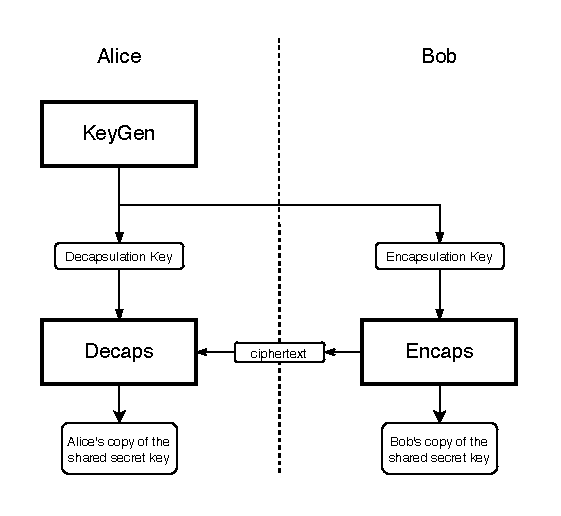
\includegraphics[width=0.5\textwidth]{doc/graph/KEM.drawio.pdf}
  \caption{KEM 工作流程图}
\end{figure}

由于 KEM 在 Decaps 阶段生成的共享密钥是确定性的,因此 KEM 通常会在 Encaps 阶段引入随机性,以避免密文的重放攻击。不同的 KEM 实现可能导致 Decaps 无法生成共享密钥,导致密文无法解密,通常会选择合适的参数,以保证发生这种情况的概率足够小。
% \section{MSKE 安全模型简述}

在密码学研究中,安全模型通常指导加密方案的设计,确保它们满足特定安全目标,并提供方案的执行框架。

Fischlin 等人在论文\cite{fischlin_multi-stage_2014}中提出多阶段密钥交换(Multi-Stage Key Exchange,MSKE)的安全模型,参考论文\cite{ideal_lattice_2023}及论文\cite{timke_2024}简要介绍如下:

MSKE 模型下参与者身份集表示为 $\mathcal{U}$,并且每一个 $U\in \mathcal{U}$ 有一个长期公钥 $\mathrm{pk}_{U}$ 和对应的私钥 $\mathrm{sk}_{U}$。 列表 $List_S$ 维护着所有会话信息,并由标签 $label$ 作为会话元组 $T$ 的唯一标识,$T$ = ($label$, $U$, $V$, $role$, $auth$, st$_\text{exec}$, $sID$, $K$, st$_{\text {key}}$, $tested$)。

其中 $U$ 与 $V$ 表示通信双方身份,
$role$ $\in\{ initiator, responder \}$ 记录会话所有者的角色。 
$auth$ 标识密钥交换协议的每个阶段的认证模式。
$\mathrm{st}_{\text{exec}}$[$label$, $i$]$\in$ \{running, accepted, rejected\} 表示在会话 $label$ 中第 $i$ 阶段的状态。 
sID 表示为针对阶段性的会话标识符,其中 $sID_i$ 表示第 $i$(非0)阶段中的会话标识符。
$K$ 表示会话 $label$ 在 $i$ 阶段中的阶段会话密钥。 
st$_\text{Key}$[$label$, $i$] $\in\{\text {fresh, revealed}\}$ 表示在会话 $label$ 中第 $i \neq 0 $ 阶段中会话(临时)密钥的状态。 
tested 记录会话密钥测试状态,$tested_i = true$ 则说明第 $i$ 阶段下的会话(临时)密钥已完成测试。

在 MSKE 安全模型下, 不允许临时密钥以及内部值(如服务器预共享密钥)泄露。 考虑一个 PPT 的敌手 $\mathcal{A}$,它控制着所有参与方之间的通信, 可以拦截、注入和丢弃消息。

\textbf{攻击手段. }敌手 $\mathcal{A}$ 通过以下查询与协议交互: 

\begin{itemize}
\setlength\itemsep{-0.3em}
\item NewSession($U$, $V$, $role$, $auth$): 为 $U$ 创建新的会话,角色为 $role$, 预期伙伴为$V$,身份验证类型 $auth$ $\in \{\text{unauth, unilateral, mutual}\}$
\item Send($label$, $m$): 发送消息$m$给标签为$label$的会话
\item Reveal($label$, $i$): 暴露$label$会话中第$i$阶段的会话密钥
\item Cor($U$): 攻陷用户$U$, 向敌手提供用户$U$长期公钥$\mathrm{pk}_{U}$ 对应的长期私钥,返回$\left(\mathrm{sk}_{U}, \mathrm{pk}_{U}\right)$
\item TEST($label$, $i$): 测试标签为 $label$ 的会话中第 $i$ 阶段的会话密钥
\end{itemize}
\subsection{TIMKE性能评估}

本节对不同配置下的TIMKE协议进行性能评估,分析各核心组件对整体性能的影响,并探讨保持安全性下的优化策略,为实际部署决策提供参考。

\subsubsection{评估方法}

实现提供一套性能评估框架,对协议各组件及其组合进行系统测试,包括:1)组件级基准测试,重点评估各KEM实现的关键操作(密钥生成、封装和解封装)性能,识别潜在瓶颈;2)协议阶段评估,分别测量第一阶段(包含0-RTT)和第二阶段的执行时间与资源消耗;3)端到端性能分析,评估完整协议流程的时间效率、内存占用和通信开销,模拟真实应用场景。替代实现对比则测试不同KEM组合的性能差异,分析最佳配置方案。

所有测试在统一的环境中进行,硬件平台为Apple M1 Pro (8核心CPU,16GB RAM),操作系统为MacOS Sequoia 15,开发语言为Go 1.23.4。每项测试重复10次取平均值,消除随机波动。测试工具集成于协议代码库,确保测量的准确性与一致性,不同身份的参与方会占用同一设备不同的端口进行交互。
重点测试两套KEM组合配置方案:1)理论构造配置使用OW-ChCCA KEM作为KEM\textsubscript{1}和ML-KEM作为KEM\textsubscript{2},代表原始TIMKE协议设计;2)实用替代配置使用ML-KEM同时作为KEM\textsubscript{1}和KEM\textsubscript{2},探索在当前技术条件下的最佳性能方案。

\subsubsection{混合KEM实现性能分析}

考虑到OW-ChCCA KEM的性能受限,首先评估折中方案:使用高度简化的OW-ChCCA变体(OWChCCA-mini)作为KEM\textsubscript{1},结合ML-KEM作为KEM\textsubscript{2}。OWChCCA-mini使用极小矩阵维度(n=16, m=8192, $\lambda$=16)和高度优化的算法实现。该配置仅作为概念验证使用,不应在实际安全系统中部署,仅提供理论构造可行性的基准数据。

\begin{table}[ht]
\centering
\caption{混合KEM实现的TIMKE协议性能(单位:毫秒)}
\label{tab:timke-hybrid-perf}
\begin{tabular}{|l|r|r|r|r|}
\hline
\textbf{KEM组合} & \textbf{阶段1} & \textbf{阶段2} & \textbf{总时间} & \textbf{内存(KB)} \\
\hline
OWChCCA-mini + ML-KEM-512    & 322.18  & 118.53  & 440.71  & 2,206,372   \\
\hline
OWChCCA-mini + ML-KEM-768    & 324.47  & 117.61  & 442.07  & 2,206,250   \\
\hline
OWChCCA-mini + ML-KEM-1024   & 374.76  & 127.47  & 502.23  & 2,204,554   \\
\hline
\end{tabular}
\end{table}

即使采用极度简化的OW-ChCCA变体,混合方案的性能仍然受到限制,不同配置总执行时间分别为440.71ms、442.07ms和502.23ms,在不稳定的网络环境下有更明显的延迟感知。第一阶段(使用OWChCCA-mini)执行时间占总时间的73\%至75\%,明确指出性能瓶颈所在。在高安全级别下更为明显,如OWChCCA-mini与ML-KEM-1024组合的配置中,第一阶段耗时达到374.76ms,几乎是第二阶段的3倍。所有混合配置均需要超过2GB的内存,远超移动设备和嵌入式系统的可用资源。较差的性能表现主要源于OWChCCA-mini中的矩阵运算,尽管较大程度的简化参数设置,但基本的LWE问题结构仍然导致过多的内存开销。

数据表明,尽管混合KEM方案在理论上实现了TIMKE协议的设计目标,但其实际性能表现使其难以直接应用于对延迟敏感的现代通信系统。

\subsubsection{ML-KEM替代实现性能分析}

本小节将分析使用ML-KEM同时替代KEM\textsubscript{1}和KEM\textsubscript{2}的方案。这种配置在理论上可能不提供与原设计相同的紧致安全保证,但为评估TIMKE协议在实际环境中的可行性提供了参考。

表\ref{tab:timke-mlkem-perf}展示了使用ML-KEM不同安全级别实现的TIMKE协议性能。

\begin{table}[ht]
\centering
\caption{基于ML-KEM的TIMKE协议性能(单位:毫秒)}
\label{tab:timke-mlkem-perf}
\begin{tabular}{|l|r|r|r|r|}
\hline
\textbf{KEM组合} & \textbf{阶段1} & \textbf{阶段2} & \textbf{总时间} & \textbf{内存(KB)} \\
\hline
ML-KEM-512 + ML-KEM-512    & 0.10  & 0.07  & 0.17  & 26   \\
\hline
ML-KEM-768 + ML-KEM-768    & 0.15  & 0.10  & 0.25  & 40   \\
\hline
ML-KEM-1024 + ML-KEM-1024  & 0.21  & 0.14  & 0.35  & 59   \\
\hline
\end{tabular}
\end{table}

在统一测试基准下,基于ML-KEM的配置比混合KEM方案快约3000倍。即使是安全级别最高的ML-KEM-1024配置,总执行时间也仅为0.35毫秒,完全满足高性能网络应用的需求。如此大的差距主要因为ML-KEM高效的算法结构和实现上的优化。ML-KEM基于模格结构,能够利用数论变换(NTT)等方式加速计算,其参数设置也经过精心优化,在保持安全的同时最小化计算开销。

内存使用方面,ML-KEM方案表现优秀。测试配置的内存消耗分别为26KB、40KB和59KB,比混合方案低4-5个数量级,使TIMKE协议能够在资源受限的环境中运行,如移动设备、物联网终端甚至某些嵌入式系统。低内存占用也意味着更低的能耗和更好的并发性能,对服务器端的部署尤为重要。

通信开销方面,基于ML-KEM的配置表现出色。ClientHello消息大小约为2-3KB,ServerResponse约为1-2KB,总通信量控制在5KB以内。阶段时间分布也更加均衡,第一阶段和第二阶段分别占总时间的约60\%和40\%。平均的时间分布在保证了0-RTT数据传输的低延迟特性的同时,不为后续阶段引入较大的额外延迟。

\paragraph{安全性降级影响分析}
从安全模型角度,OW-ChCCA安全专为紧致安全多挑战多用户场景设计,其安全损失与用户数量$n$和会话数量$q_s$无关,安全规约损失为常数$\mathcal{O}(1)$。ML-KEM虽然提供了IND-CCA2安全,但在多用户环境下其安全损失会随用户数量增加,典型的安全损失为$\mathcal{O}(n \cdot q_s)$。
对于小规模系统(如用户数$n < 10^3$,每用户会话数$q_s < 10^3$),ML-KEM配置下的安全性损失可接受,实际参数选择与理论安全级别差距可控;对于中等规模系统(如用户数$n \approx 10^6$,每用户会话数$q_s \approx 10^3$),安全损失达到$\mathcal{O}(10^9)$量级,需要增加密钥长度(约30比特)才能维持原有安全级别;对于大规模系统(如用户数$n > 10^8$,每用户会话数$q_s > 10^4$),安全损失将超过$\mathcal{O}(10^{12})$量级,安全参数增加需求可能使方案在计算和通信效率上不再具有实用性。

使用ML-KEM替代OW-ChCCA KEM作为KEM\textsubscript{1}会对TIMKE协议的整体安全性产生影响,具体如下:

\begin{enumerate}
    \item \textbf{紧致安全性}:完全失去紧致安全保证,安全损失会随系统规模增长。
    
    \item \textbf{后量子安全性}:保持不变,ML-KEM本身具有抗量子计算攻击能力。
    
    \item \textbf{0-RTT安全性}:基本保持,但在大规模部署中,可能需要增加密钥长度以补偿安全损失。
    
    \item \textbf{弱前向安全性}:第二阶段的弱前向安全性基本保持,因为它主要依赖于KEM\textsubscript{2}的安全性。
\end{enumerate}

综合来看,ML-KEM替代方案在部署TIMKE协议的中小规模系统中可以接受,安全降级影响有限。大规模部署环境则需权衡效率与安全性,可能要求更高安全级别的参数以补偿紧致安全性的损失。 % 附录
\thispagestyle{empty}

\begin{center}
  \zihao{0}
  \textbf{华南师范大学}
\end{center}

\begin{center}
\zihao{0}
\textbf{本科毕业论文 (设计)}
\end{center}

\begin{center}
\zihao{1}
\ \\
\end{center}

\begin{table}[ht]
  \zihao{2}
  \setlength\extrarowheight{10pt}
  \centering
  \begin{tabular}{lc}
  \textbf{题\ 目:}  & \textbf{短的论文题目一行}            \\ \cline{2-2}
  \textbf{}  & \textbf{长的论文题目两行}            \\ \cline{2-2}
  \end{tabular}
\end{table}

\begin{center}
\zihao{1}
\ \\\ \\\ \\
\end{center}
\begin{spacing}{1.8}

\begin{table}[ht]
  \zihao{-3}
  \setlength\extrarowheight{10pt}
  \centering
  \begin{tabular}{lc}
  \textbf{姓\ 名:}  & \textbf{你的名字}             \\ \cline{2-2} 
  \textbf{学\ 号:}  & \textbf{20152100001}     \\ \cline{2-2} 
  \textbf{系\ 别:}  & \textbf{计算机系}            \\ \cline{2-2} 
  \textbf{专业班级:\ } & \textbf{计算机科学与技术 (网络工程)} \\ \cline{2-2} 
  \textbf{指导老师:\ } & \textbf{指导老师}             \\ \cline{2-2} 
  \multicolumn{2}{c}{\textbf{2019年4月2日}}   
  \end{tabular}
\end{table}

\end{spacing}
\afterpage{\blankpage}
\newpage % 致谢
\end{spacing}

% 结束计算页码
\setboolean{@twoside}{false}

\end{document}